\documentclass[12pt, a4paper]{article}

\usepackage[dvips]{graphics}
\usepackage{tabularx}
\usepackage{amsmath}
\usepackage{amsfonts}
\usepackage{amssymb}
\usepackage{graphicx}
\usepackage{float}
\usepackage{listings}
\usepackage{rotating}
\usepackage{tikz}
\usepackage{verbatim}
\pdfgentounicode=1

\begin{document}

\title{The FMB algorithm\\An intersection detection algorithm for 2D/3D cuboid and tetrahedron based on the Fourier-Motzkin elimination method}
\author{P. Baillehache}
\date{\today}
\maketitle

\begin{abstract}
In this paper I introduce how to perform intersection detection of pair of cuboid/tetrahedron in 2D and 3D by using the Fourier-Motzkin elimination method. The mathematical definition and solution of the problem in the two first sections is followed by the algorithm of the solution and its implementation in the C programming language in the two following sections. The last two sections introduce the validation and qualification of the FMB algorithm against the SAT algorithm.
\end{abstract}

\newpage
\tableofcontents

\section{Notations}

\begin{itemize}
\item{$\left[M\right]_{r,c}$ is the component at column $c$ and row $r$ of the matrix $M$}
\item{$\left[V\right]_r$ is the $r$-th component of the vector $\overrightarrow{V}$}
\end{itemize}

\section{Definition of the problem}

\subsection{Static case}

In this paper I'll use the term "Frame" to speak indifferently of cuboid and tetrahedron.\\

The two Frames are represented as a vector origin and a number of component vectors equal to the dimension $D$ of the space where live the Frames. Each vector is of dimension equal to $D$.\\

Lets call $\mathbb{A}$ and $\mathbb{B}$ the two Frames tested for intersection. If $A$ and $B$ are two cuboids:
\begin{equation}
\mathbb{A}=\left\lbrace
\begin{array}{c}
\overrightarrow{X}\in[0.0,1.0]^D\\
\overrightarrow{O_\mathbb{A}}+C_\mathbb{A}.\overrightarrow{X}
\end{array}
\right\rbrace
\end{equation}
\begin{equation}
\mathbb{B}=\left\lbrace
\begin{array}{c}
\overrightarrow{X}\in[0.0,1.0]^D\\
\overrightarrow{O_\mathbb{B}}+C_\mathbb{B}.\overrightarrow{X}
\end{array}
\right\rbrace
\end{equation}
where $\overrightarrow{O_\mathbb{A}}$ is the origin of $\mathbb{A}$ and $C_\mathbb{A}$ is the matrix of the components of $A$ (one component per column). Idem for $\overrightarrow{O_\mathbb{B}}$ and $C_\mathbb{B}$.\\

If $\mathbb{A}$ and $\mathbb{B}$ are two tetrahedrons:
\begin{equation}
\mathbb{A}=\left\lbrace
\begin{array}{c}
\overrightarrow{X}\in[0.0,1.0]^D\\
\sum_{i=0}^{D-1}\left[X\right]_i\le1.0\\
\overrightarrow{O_\mathbb{A}}+C_\mathbb{A}.\overrightarrow{X}
\end{array}
\right\rbrace
\end{equation}
\begin{equation}
\mathbb{B}=\left\lbrace
\begin{array}{c}
\overrightarrow{X}\in[0.0,1.0]^D\\
\sum_{i=0}^{D-1}\left[X\right]_i\le1.0\\
\overrightarrow{O_\mathbb{B}}+C_\mathbb{B}.\overrightarrow{X}
\end{array}
\right\rbrace
\end{equation}

I'll assume the Frames are well formed, i.e. their components matrix is invertible. It is then possible to express $\mathbb{B}$ in $\mathbb{A}$'s coordinates system, noted as $\mathbb{B}_\mathbb{A}$. If $\mathbb{B}$ is a cuboid:
\begin{equation}
\mathbb{B}_\mathbb{A}=\left\lbrace
\begin{array}{c}
\overrightarrow{X}\in[0.0,1.0]^D\\
C_\mathbb{A}^{-1}.(\overrightarrow{O_\mathbb{B}}-\overrightarrow{O_\mathbb{A}}+C_\mathbb{B}.\overrightarrow{X})
\end{array}
\right\rbrace
\end{equation}

If $\mathbb{B}$ is a tetrahedron:
\begin{equation}
\mathbb{B}_\mathbb{A}=\left\lbrace
\begin{array}{c}
\overrightarrow{X}\in[0.0,1.0]^D\\
\sum_{i=0}^{D-1}\left[X\right]_i\le1.0\\
C_\mathbb{A}^{-1}.(\overrightarrow{O_\mathbb{B}}-\overrightarrow{O_\mathbb{A}}+C_\mathbb{B}.\overrightarrow{X})
\end{array}
\right\rbrace
\end{equation}

$\mathbb{A}$ in its own coordinates system becomes, for a cuboid:
\begin{equation}
\mathbb{A}_\mathbb{A}=\left\lbrace\overrightarrow{X}\in[0.0,1.0]^D\right\rbrace
\end{equation}
and for a tetrahedron:
\begin{equation}
\mathbb{A}_\mathbb{A}=\left\lbrace
\begin{array}{c}
\overrightarrow{X}\in[0.0,1.0]^D\\
\sum_{i=0}^{D-1}\left[X\right]_i\le1.0
\end{array}
\right\rbrace
\end{equation}

The intersection of $\mathbb{A}$ and $\mathbb{B}$ in $\mathbb{A}$'s coordinates sytem, can then be expressed as follow.\\

If $\mathbb{A}$ and $\mathbb{B}$ are two cuboids:
\begin{equation}
\left\lbrace
\begin{array}{c}
\overrightarrow{X}\in[0.0,1.0]^D\\
C_\mathbb{A}^{-1}.\left(\overrightarrow{O_\mathbb{B}}-\overrightarrow{O_\mathbb{A}}+C_\mathbb{B}.\overrightarrow{X}\right)\cap[0.0,1.0]^D
\end{array}
\right\rbrace
\end{equation}

If $\mathbb{A}$ is a cuboid and $\mathbb{B}$ is a tetrahedron:
\begin{equation}
\left\lbrace
\begin{array}{c}
\overrightarrow{X}\in[0.0,1.0]^D\\
\sum_{i=0}^{D-1}\left[X\right]_i\le1.0\\
C_\mathbb{A}^{-1}.\left(\overrightarrow{O_\mathbb{B}}-\overrightarrow{O_\mathbb{A}}+C_\mathbb{B}.\overrightarrow{X}\right)\cap[0.0,1.0]^D
\end{array}
\right\rbrace
\end{equation}

If $\mathbb{A}$ is a tetrahedron and $\mathbb{B}$ is a cuboid:
\begin{equation}
\left\lbrace
\begin{array}{c}
\overrightarrow{X}\in[0.0,1.0]^D\\
C_\mathbb{A}^{-1}.\left(\overrightarrow{O_\mathbb{B}}-\overrightarrow{O_\mathbb{A}}+C_\mathbb{B}.\overrightarrow{X}\right)\cap[0.0,1.0]^D\\
\sum_{i=0}^{D-1}\left[C_\mathbb{A}^{-1}.\left(\overrightarrow{O_\mathbb{B}}-\overrightarrow{O_\mathbb{A}}+C_\mathbb{B}.\overrightarrow{X}\right)\right]_i\le1.0\\
\end{array}
\right\rbrace
\end{equation}

If $\mathbb{A}$ and $\mathbb{B}$ are two tetrahedrons:
\begin{equation}
\left\lbrace
\begin{array}{c}
\overrightarrow{X}\in[0.0,1.0]^D\\
\sum_{i=0}^{D-1}\left[X\right]_i\le1.0\\
C_\mathbb{A}^{-1}.(\overrightarrow{O_\mathbb{B}}-\overrightarrow{O_\mathbb{A}}+C_\mathbb{B}.\overrightarrow{X})\cap[0.0,1.0]^D\\
\sum_{i=0}^{D-1}\left[C_\mathbb{A}^{-1}.\left(\overrightarrow{O_\mathbb{B}}-\overrightarrow{O_\mathbb{A}}+C_\mathbb{B}.\overrightarrow{X}\right)\right]_i\le1.0\\
\end{array}
\right\rbrace
\end{equation}

These can in turn be expressed as systems of linear inequations as follows, given the two shortcuts $\overrightarrow{O_{\mathbb{B}_\mathbb{A}}}=C_\mathbb{A}^{-1}.(\overrightarrow{O_\mathbb{B}}-\overrightarrow{O_\mathbb{A}})$ and $C_{\mathbb{B}_\mathbb{A}}=C_\mathbb{A}^{-1}.C_{\mathbb{B}}$.

If $\mathbb{A}$ and $\mathbb{B}$ are two cuboids:
\begin{equation}
\left\lbrace
\begin{array}{rcl}
\left[X\right]_0&\le&1.0\\
-\left[X\right]_0&\le&0.0\\
...\\
\left[X\right]_{D-1}&\le&1.0\\
-\left[X\right]_{D-1}&\le&0.0\\
\sum_{i=0}^{D-1}\left[C_{\mathbb{B}_\mathbb{A}}\right]_{0,i}.\left[X\right]_i&\le&1.0-\left[O_{\mathbb{B}_\mathbb{A}}\right]_0\\
-\sum_{i=0}^{D-1}\left[C_{\mathbb{B}_\mathbb{A}}\right]_{0,i}.\left[X\right]_i&\le&-\left[O_{\mathbb{B}_\mathbb{A}}\right]_0\\
...\\
\sum_{i=0}^{D-1}\left[C_{\mathbb{B}_\mathbb{A}}\right]_{D-1,i}.\left[X\right]_i&\le&1.0-\left[O_{\mathbb{B}_\mathbb{A}}\right]_{D-1}\\
-\sum_{i=0}^{D-1}\left[C_{\mathbb{B}_\mathbb{A}}\right]_{D-1,i}.\left[X\right]_i&\le&-\left[O_{\mathbb{B}_\mathbb{A}}\right]_{D-1}
\end{array}
\right.
\end{equation}

If $\mathbb{A}$ is a cuboid and $\mathbb{B}$ is a tetrahedron:
\begin{equation}
\left\lbrace
\begin{array}{rcl}
-\left[X\right]_0&\le&0.0\\
...\\
-\left[X\right]_{D-1}&\le&0.0\\
\sum_{i=0}^{D-1}\left[C_{\mathbb{B}_\mathbb{A}}\right]_{0,i}.\left[X\right]_i&\le&1.0-\left[O_{\mathbb{B}_\mathbb{A}}\right]_0\\
-\sum_{i=0}^{D-1}\left[C_{\mathbb{B}_\mathbb{A}}\right]_{0,i}.\left[X\right]_i&\le&-\left[O_{\mathbb{B}_\mathbb{A}}\right]_0\\
...\\
\sum_{i=0}^{D-1}\left[C_{\mathbb{B}_\mathbb{A}}\right]_{D-1,i}.\left[X\right]_i&\le&1.0-\left[O_{\mathbb{B}_\mathbb{A}}\right]_{D-1}\\
-\sum_{i=0}^{D-1}\left[C_{\mathbb{B}_\mathbb{A}}\right]_{D-1,i}.\left[X\right]_i&\le&-\left[O_{\mathbb{B}_\mathbb{A}}\right]_{D-1}\\
\sum_{i=0}^{D-1}\left[X\right]_i&\le&1.0
\end{array}
\right.
\end{equation}

If $\mathbb{A}$ is a tetrahedron and $\mathbb{B}$ is a cuboid:
\begin{equation}
\left\lbrace
\begin{array}{rcl}
\left[X\right]_0&\le&1.0\\
-\left[X\right]_0&\le&0.0\\
...\\
\left[X\right]_{D-1}&\le&1.0\\
-\left[X\right]_{D-1}&\le&0.0\\
-\sum_{i=0}^{D-1}\left[C_{\mathbb{B}_\mathbb{A}}\right]_{0,i}.\left[X\right]_i&\le&-\left[O_{\mathbb{B}_\mathbb{A}}\right]_0\\
...\\
\sum_{i=0}^{D-1}\left[C_{\mathbb{B}_\mathbb{A}}\right]_{D-1,i}.\left[X\right]_i&\le&1.0-\left[O_{\mathbb{B}_\mathbb{A}}\right]_{D-1}\\
-\sum_{i=0}^{D-1}\left[C_{\mathbb{B}_\mathbb{A}}\right]_{D-1,i}.\left[X\right]_i&\le&-\left[O_{\mathbb{B}_\mathbb{A}}\right]_{D-1}\\
\sum_{j=0}^{D-1}\left(\left(\sum_{i=0}^{D-1}\left[C_{\mathbb{B}_\mathbb{A}}\right]_{j,i}\right).\left[X\right]_i\right)&\le&1.0-\sum_{i=0}^{D-1}\left[O_{\mathbb{B}_\mathbb{A}}\right]_i
\end{array}
\right.
\end{equation}

If $\mathbb{A}$ and $\mathbb{B}$ are two tetrahedrons:
\begin{equation}
\left\lbrace
\begin{array}{rcl}
-\left[X\right]_0&\le&0.0\\
...\\
-\left[X\right]_{D-1}&\le&0.0\\
-\sum_{i=0}^{D-1}\left[C_{\mathbb{B}_\mathbb{A}}\right]_{0,i}.\left[X\right]_i&\le&-\left[O_{\mathbb{B}_\mathbb{A}}\right]0}\\
...\\
\sum_{i=0}^{D-1}\left[C_{\mathbb{B}_\mathbb{A}}\right]_{D-1,i}.\left[X\right]_i&\le&1.0-\left[O_{\mathbb{B}_\mathbb{A}}\right]_{D-1}\\
-\sum_{i=0}^{D-1}\left[C_{\mathbb{B}_\mathbb{A}}\right]_{D-1,i}.\left[X\right]_i&\le&-\left[O_{\mathbb{B}_\mathbb{A}}\right]_{D-1}\\
\sum_{i=0}^{D-1}\left[X\right]_i&\le&1.0\\
\sum_{j=0}^{D-1}\left(\left(\sum_{i=0}^{D-1}\left[C_{\mathbb{B}_\mathbb{A}}\right]_{j,i}\right).\left[X\right]_i\right)&\le&1.0-\sum_{i=0}^{D-1}\left[O_{\mathbb{B}_\mathbb{A}}\right]_i
\end{array}
\right.
\end{equation}

\subsection{Dynamic case}

If the frames $\mathbb{A}$ and $\mathbb{B}$ are moving linearly along the vectors $\overrightarrow{V_\mathbb{A}}$ and $\overrightarrow{V_\mathbb{B}}$ respectively during the interval of time $t\in[0.0,1.0]$, the above definition of the problem is modified as follow.\\

If $A$ and $B$ are two cuboids:
\begin{equation}
\mathbb{A}=\left\lbrace
\begin{array}{c}
\overrightarrow{X}\in[0.0,1.0]^D\\
t\in[0.0,1.0]\\
\overrightarrow{O_\mathbb{A}}+C_\mathbb{A}.\overrightarrow{X}+\overrightarrow{V_\mathbb{A}}.t
\end{array}
\right\rbrace
\end{equation}
\begin{equation}
\mathbb{B}=\left\lbrace
\begin{array}{c}
\overrightarrow{X}\in[0.0,1.0]^D\\
t\in[0.0,1.0]\\
\overrightarrow{O_\mathbb{B}}+C_\mathbb{B}.\overrightarrow{X}+\overrightarrow{V_\mathbb{B}}.t
\end{array}
\right\rbrace
\end{equation}
where $\overrightarrow{O_\mathbb{A}}$ is the origin of $\mathbb{A}$ and $C_\mathbb{A}$ is the matrix of the components of $A$ (one component per column). Idem for $\overrightarrow{O_\mathbb{B}}$ and $C_\mathbb{B}$.\\

If $\mathbb{A}$ and $\mathbb{B}$ are two tetrahedrons:
\begin{equation}
\mathbb{A}=\left\lbrace
\begin{array}{c}
\overrightarrow{X}\in[0.0,1.0]^D\\
t\in[0.0,1.0]\\
\sum_{i=0}^{D-1}\left[X\right]_i\le1.0\\
\overrightarrow{O_\mathbb{A}}+C_\mathbb{A}.\overrightarrow{X}+\overrightarrow{V_\mathbb{A}}.t
\end{array}
\right\rbrace
\end{equation}
\begin{equation}
\mathbb{B}=\left\lbrace
\begin{array}{c}
\overrightarrow{X}\in[0.0,1.0]^D\\
t\in[0.0,1.0]\\
\sum_{i=0}^{D-1}\left[X\right]_i\le1.0\\
\overrightarrow{O_\mathbb{B}}+C_\mathbb{B}.\overrightarrow{X}+\overrightarrow{V_\mathbb{B}}.t
\end{array}
\right\rbrace
\end{equation}

If $\mathbb{B}$ is a cuboid, $\mathbb{B}_\mathbb{A}$ becomes:
\begin{equation}
\mathbb{B}_\mathbb{A}=\left\lbrace
\begin{array}{c}
\overrightarrow{X}\in[0.0,1.0]^D\\
t\in[0.0,1.0]\\
C_\mathbb{A}^{-1}.\left(\overrightarrow{O_\mathbb{B}}-\overrightarrow{O_\mathbb{A}}+C_\mathbb{B}.\overrightarrow{X}+\left(\overrightarrow{V_\mathbb{B}}-\overrightarrow{V_\mathbb{A}}\right).t\right)
\end{array}
\right\rbrace
\end{equation}

If $\mathbb{B}$ is a tetrahedron:
\begin{equation}
\mathbb{B}_\mathbb{A}=\left\lbrace
\begin{array}{c}
\overrightarrow{X}\in[0.0,1.0]^D\\
t\in[0.0,1.0]\\
\sum_{i=0}^{D-1}\left[X\right]_i\le1.0\\
C_\mathbb{A}^{-1}.\left(\overrightarrow{O_\mathbb{B}}-\overrightarrow{O_\mathbb{A}}+C_\mathbb{B}.\overrightarrow{X}+\left(\overrightarrow{V_\mathbb{B}}-\overrightarrow{V_\mathbb{A}}\right).t\right)
\end{array}
\right\rbrace
\end{equation}

$\mathbb{A}$ in its own coordinates system has the same definition as in the static case. For a cuboid:
\begin{equation}
\mathbb{A}_\mathbb{A}=\left\lbrace\overrightarrow{X}\in[0.0,1.0]^D\right\rbrace
\end{equation}
and for a tetrahedron:
\begin{equation}
\mathbb{A}_\mathbb{A}=\left\lbrace
\begin{array}{c}
\overrightarrow{X}\in[0.0,1.0]^D\\
\sum_{i=0}^{D-1}\left[X\right]_i\le1.0\end{array}
\right\rbrace
\end{equation}

The intersection of $\mathbb{A}$ and $\mathbb{B}$ in $\mathbb{A}$'s coordinates sytem, can then be expressed as follow.\\

If $\mathbb{A}$ and $\mathbb{B}$ are two cuboids:
\begin{equation}
\left\lbrace
\begin{array}{c}
\overrightarrow{X}\in[0.0,1.0]^D\\
t\in[0.0,1.0]\\
C_\mathbb{A}^{-1}.\left(\overrightarrow{O_\mathbb{B}}-\overrightarrow{O_\mathbb{A}}+C_\mathbb{B}.\overrightarrow{X}+\left(\overrightarrow{V_\mathbb{B}}-\overrightarrow{V_\mathbb{A}}\right).t\right)\cap[0.0,1.0]^D
\end{array}
\right\rbrace
\end{equation}

If $\mathbb{A}$ is a cuboid and $\mathbb{B}$ is a tetrahedron:
\begin{equation}
\left\lbrace
\begin{array}{c}
\overrightarrow{X}\in[0.0,1.0]^D\\
t\in[0.0,1.0]\\
\sum_{i=0}^{D-1}\left[X\right]_i\le1.0\\
C_\mathbb{A}^{-1}.\left(\overrightarrow{O_\mathbb{B}}-\overrightarrow{O_\mathbb{A}}+C_\mathbb{B}.\overrightarrow{X}+\left(\overrightarrow{V_\mathbb{B}}-\overrightarrow{V_\mathbb{A}}\right).t\right)\cap[0.0,1.0]^D
\end{array}
\right\rbrace
\end{equation}

If $\mathbb{A}$ is a tetrahedron and $\mathbb{B}$ is a cuboid:
\begin{equation}
\left\lbrace
\begin{array}{c}
\overrightarrow{X}\in[0.0,1.0]^D\\
t\in[0.0,1.0]\\
C_\mathbb{A}^{-1}.\left(\overrightarrow{O_\mathbb{B}}-\overrightarrow{O_\mathbb{A}}+C_\mathbb{B}.\overrightarrow{X}+\left(\overrightarrow{V_\mathbb{B}}-\overrightarrow{V_\mathbb{A}}\right).t\right)\cap[0.0,1.0]^D\\
\sum_{i=0}^{D-1}\left[C_\mathbb{A}^{-1}.\left(\overrightarrow{O_\mathbb{B}}-\overrightarrow{O_\mathbb{A}}+C_\mathbb{B}.\overrightarrow{X}\right)\right]_i\le1.0\\
\end{array}
\right\rbrace
\end{equation}

If $\mathbb{A}$ and $\mathbb{B}$ are two tetrahedrons:
\begin{equation}
\left\lbrace
\begin{array}{c}
\overrightarrow{X}\in[0.0,1.0]^D\\
t\in[0.0,1.0]\\
\sum_{i=0}^{D-1}\left[X\right]_i\le1.0\\
C_\mathbb{A}^{-1}.\left(\overrightarrow{O_\mathbb{B}}-\overrightarrow{O_\mathbb{A}}+C_\mathbb{B}.\overrightarrow{X}+\left(\overrightarrow{V_\mathbb{B}}-\overrightarrow{V_\mathbb{A}}\right).t\right)\cap[0.0,1.0]^D\\
\sum_{i=0}^{D-1}\left[C_\mathbb{A}^{-1}.\left(\overrightarrow{O_\mathbb{B}}-\overrightarrow{O_\mathbb{A}}+C_\mathbb{B}.\overrightarrow{X}\right)\right]_i\le1.0\\
\end{array}
\right\rbrace
\end{equation}

These lead to the systems of linear inequations as follows, given the three shortcuts $\overrightarrow{O_{\mathbb{B}_\mathbb{A}}}=C_\mathbb{A}^{-1}.(\overrightarrow{O_\mathbb{B}}-\overrightarrow{O_\mathbb{A}})$, $\overrightarrow{V_{\mathbb{B}_\mathbb{A}}}=C_\mathbb{A}^{-1}.(\overrightarrow{V_\mathbb{B}}-\overrightarrow{V_\mathbb{A}})$ and $C_{\mathbb{B}_\mathbb{A}}=C_\mathbb{A}^{-1}.C_{\mathbb{B}}$.

If $\mathbb{A}$ and $\mathbb{B}$ are two cuboids:
\begin{equation}
\left\lbrace
\begin{array}{rcl}
t&\le&1.0\\
-t&\le&0.0\\
\left[X\right]_0&\le&1.0\\
-\left[X\right]_0&\le&0.0\\
...\\
\left[X\right]_{D-1}&\le&1.0\\
-\left[X\right]_{D-1}&\le&0.0\\
\left[V_{\mathbb{B}_\mathbb{A}}\right]_0t+\sum_{i=0}^{D-1}\left[C_{\mathbb{B}_\mathbb{A}}\right]_{0,i}\left[X\right]_i&\le&1.0-\left[O_{\mathbb{B}_\mathbb{A}}\right]_0\\
-\left[V_{\mathbb{B}_\mathbb{A}}\right]_0t-\sum_{i=0}^{D-1}\left[C_{\mathbb{B}_\mathbb{A}}\right]_{0,i}\left[X\right]_i&\le&-\left[O_{\mathbb{B}_\mathbb{A}}\right]_0\\
...\\
\left[V_{\mathbb{B}_\mathbb{A}}\right]_{D-1}t+\sum_{i=0}^{D-1}\left[C_{\mathbb{B}_\mathbb{A}}\right]_{D-1,i}\left[X\right]_i&\le&1.0-\left[O_{\mathbb{B}_\mathbb{A}}\right]_{D-1}\\
-\left[V_{\mathbb{B}_\mathbb{A}}\right]_{D-1}t-\sum_{i=0}^{D-1}\left[C_{\mathbb{B}_\mathbb{A}}\right]_{D-1,i}\left[X\right]_i&\le&-\left[O_{\mathbb{B}_\mathbb{A}}\right]_{D-1}
\end{array}
\right.
\end{equation}

If $\mathbb{A}$ is a cuboid and $\mathbb{B}$ is a tetrahedron:
\begin{equation}
\left\lbrace
\begin{array}{rcl}
t&\le&1.0\\
-t&\le&0.0\\
-\left[X\right]_0&\le&0.0\\
...\\
-\left[X\right]_{D-1}&\le&0.0\\
\sum_{i=0}^{D-1}\left[C_{\mathbb{B}_\mathbb{A}}\right]_{0,i}\left[X\right]_i&\le&1.0-\left[O_{\mathbb{B}_\mathbb{A}}\right]_0\\
-\sum_{i=0}^{D-1}\left[C_{\mathbb{B}_\mathbb{A}}\right]_{0,i}\left[X\right]_i&\le&-\left[O_{\mathbb{B}_\mathbb{A}}\right]_0\\
...\\
\left[V_{\mathbb{B}_\mathbb{A}}\right]_{D-1}t+\sum_{i=0}^{D-1}\left[C_{\mathbb{B}_\mathbb{A}}\right]_{D-1,i}\left[X\right]_i&\le&1.0-\left[O_{\mathbb{B}_\mathbb{A}}\right]_{D-1}\\
-\left[V_{\mathbb{B}_\mathbb{A}}\right]_{D-1}t-\sum_{i=0}^{D-1}\left[C_{\mathbb{B}_\mathbb{A}}\right]_{D-1,i}\left[X\right]_i&\le&-\left[O_{\mathbb{B}_\mathbb{A}}\right]_{D-1}\\
\sum_{i=0}^{D-1}\left[X\right]_i&\le&1.0
\end{array}
\right.
\end{equation}

If $\mathbb{A}$ is a tetrahedron and $\mathbb{B}$ is a cuboid:
\begin{equation}
\left\lbrace
\begin{array}{rcl}
t&\le&1.0\\
-t&\le&0.0\\
\left[X\right]_0&\le&1.0\\
-\left[X\right]_0&\le&0.0\\
...\\
\left[X\right]_{D-1}&\le&1.0\\
-\left[X\right]_{D-1}&\le&0.0\\
-\sum_{i=0}^{D-1}\left[C_{\mathbb{B}_\mathbb{A}}\right]_{0,i}\left[X\right]_i&\le&-\left[O_{\mathbb{B}_\mathbb{A}}\right]_0\\
...\\
\left[V_{\mathbb{B}_\mathbb{A}}\right]_{D-1}t+\sum_{i=0}^{D-1}\left[C_{\mathbb{B}_\mathbb{A}}\right]_{D-1,i}\left[X\right]_i&\le&1.0-\left[O_{\mathbb{B}_\mathbb{A}}\right]_{D-1}\\
-\left[V_{\mathbb{B}_\mathbb{A}}\right]_{D-1}t-\sum_{i=0}^{D-1}\left[C_{\mathbb{B}_\mathbb{A}}\right]_{D-1,i}\left[X\right]_i&\le&-\left[O_{\mathbb{B}_\mathbb{A}}\right]_{D-1}\\
\sum_{j=0}^{D-1}\left(\left(\sum_{i=0}^{D-1}\left[C_{\mathbb{B}_\mathbb{A}}\right]_{j,i}\right)\left[X\right]_i\right)&\le&1.0-\sum_{i=0}^{D-1}\left[O_{\mathbb{B}_\mathbb{A}}\right]_{i}
\end{array}
\right.
\end{equation}

If $\mathbb{A}$ and $\mathbb{B}$ are two tetrahedrons:
\begin{equation}
\left\lbrace
\begin{array}{rcl}
t&\le&1.0\\
-t&\le&0.0\\
-\left[X\right]_0&\le&0.0\\
...\\
-\left[X\right]_{D-1}&\le&0.0\\
-\sum_{i=0}^{D-1}\left[C_{\mathbb{B}_\mathbb{A}}\right]_{0,i}\left[X\right]_i&\le&-\left[O_{\mathbb{B}_\mathbb{A}}\right]_{0}\\
...\\
\left[V_{\mathbb{B}_\mathbb{A}}\right]_{D-1}t+\sum_{i=0}^{D-1}\left[C_{\mathbb{B}_\mathbb{A}}\right]_{D-1,i}\left[X\right]_i&\le&1.0-\left[O_{\mathbb{B}_\mathbb{A}}\right]_{D-1}\\
-\left[V_{\mathbb{B}_\mathbb{A}}\right]_{D-1}t-\sum_{i=0}^{D-1}\left[C_{\mathbb{B}_\mathbb{A}}\right]_{D-1,i}\left[X\right]_i&\le&-\left[O_{\mathbb{B}_\mathbb{A}}\right]_{D-1}\\
\sum_{i=0}^{D-1}\left[X\right]_i&\le&1.0\\
\sum_{j=0}^{D-1}\left(\left(\sum_{i=0}^{D-1}\left[C_{\mathbb{B}_\mathbb{A}}\right]_{j,i}\right)\left[X\right]_i\right)&\le&1.0-\sum_{i=0}^{D-1}\left[O_{\mathbb{B}_\mathbb{A}}\right]_{i}
\end{array}
\right.
\end{equation}





\section{Solution}

\subsection{Fourier-Motzkin elimination method}

The Fourier-Motzkin elimination method has been introduced by J.J.-B. Fourier in 1827 \cite{fourier}, and described in the Ph.D. thesis of T.S. Motzkin in 1936 \cite{motzkin}. This is a generalization of the Gaussian elimination method to linear systems of inequalities. This method consists of eliminating one variable of the system and rewrite a new system accordingly. Then the elimination operation is repeated on another variable in the new system, and so on until we obtain a trivial system with only one variable. From there, a solution for each variable can be obtained if it exists. The variable elimination is performed as follow.\\
Lets write the linear system $\mathcal{I}$ of $m$ inequalities and $n$ variables as 
\begin{equation}
\left\{\
\begin{array}{ccccc}
a_{11}.x_1&+a_{12}.x_2&+\cdots&+a_{1n}.x_n &\le b_1\\
a_{21}.x_1&+a_{22}.x_2&+\cdots&+a_{2n}.x_n &\le b_2\\
&&\vdots&&\\
a_{m1}.x_1&+a_{m2}.x_2&+\cdots&+a_{mn}.x_n &\le b_m\\
\end{array}
\right.
\end{equation}
with
\begin{equation}
\begin{array}{c}
i\in{1, 2, ..., m}\\
j\in{1, 2, ..., n}\\
x_i\in\mathbb{R}\\
a_{ij}\in\mathbb{R}\\
b_j\in\mathbb{R} 
\end{array}
\end{equation}
To eliminate the first variable $x_1$, lets multiply each inequality by $1.0/|a_{i1}|$ where $a_{i1}\not=0.0$. The system becomes
\begin{equation}
\left\{\
\begin{array}{ccccc}
x_1&+a'_{i2}.x_2&+\cdots&+a'_{in}.x_n &\le b'_i\qquad(i\in\mathcal{I}_+)\\
&a_{i2}.x_2&+\cdots&+a_{in}.x_n &\le b_i\qquad(i\in\mathcal{I}_0)\\
-x_1&+a'_{i2}.x_2&+\cdots&+a'_{in}.x_n &\le b'_i\qquad(i\in\mathcal{I}_-)\\
\end{array}
\right.
\end{equation}
where 
$$\mathcal{I}_+=\{i:a_{i1}>0.0\}$$
$$\mathcal{I}_0=\{i:a_{i1}=0.0\}$$
$$\mathcal{I}_-=\{i:a_{i1}<0.0\}$$
$$a'_{ij}=a_{ij}/|a_{i1}|$$
$$b'_i=b_i/|a_{i1}|$$
Then $x_1, x_2, \cdots, x_n\in\mathbb{R}^n$ is a solution of $\mathcal{I}$ if and only if
\begin{equation}
\left\{\
\begin{array}{c}
\sum_{j=2}^n((a'_{kj}+a'_{lj}).x_j)\le b'_k+b'_l \qquad (k\in\mathcal{I}_+, l\in\mathcal{I}_-)\\
\sum_{j=2}^n(a_{ij}.x_j)\le b_i \qquad i\in\mathcal{I}_0
\end{array}
\right.
\end{equation}
and
\begin{equation}
\max_{l\in\mathcal{I}_-}(\sum_{j=2}^n(a'_{lj}.x_j)-b'_l)\le x_1\le\min_{k\in\mathcal{I}_+}(b'_k-\sum_{j=2}^n(a'_{kj}.x_j))
\end{equation}
The same method is then applied on this new system to eliminate the second variable $x_2$, and so on until we reach the inequality
\begin{equation}
\max_{l\in\mathcal{I}^{''...'}_-}(-b^{''...'}_l)\le x_n\le\min_{k\in\mathcal{I}^{''...'}_+}(b^{''...'}_k)
\end{equation}
If this inequality has no solution, then neither the system $\mathcal{I}$. If it has a solution, the minimum and maximum are the bounding values for the variable $x_n$. One can get a particular solution to the system $\mathcal{I}$ by choosing a value for $x_n$ between these bounding values, which allow us to set a particular value for the variable $x_{n-1}$, and so on back up to $x_1$. 

\subsection{Application of the Fourier-Motzkin method to the intersection problem}

The Fourier-Motzkin method can be directly applied to obtain the bounds of each variable, if the system has a solution. If the system has no solution, the method will eventually reach an inconsistent inequality.\\

One solution $\overrightarrow{S}$ within the bounds obtained by the resolution of the system is expressed in the Frame $\mathbb{B}$'s coordinates system. One can get the equivalent coordinates $\overrightarrow{S'}$ in the real world's coordinates system as follow:
\begin{equation}
\overrightarrow{S'}=\overrightarrow{O_\mathbb{B}}+C_\mathbb{B}.\overrightarrow{S}
\end{equation}

Only one inconsistent inequality is sufficient to prove the absence of solution, and then the non intersection of the Frames. One shall check the inconsistence of each inequality as soon as possible during the resolution of the system to optimize the speed of the algorithm.\\

A suficient condition for one inequality $\sum_ia_iX_i\le Y$ to be inconsistent is, given that $\forall i,X_i\in[0.0,1.0]$:
\begin{equation}
Y<\sum_{i\in I^-}a_i
\end{equation}
where $I^-=\left\lbrace i, a_i<0.0\right\rbrace$.\\

\section{Algorithms}

In this section I introduce the algorithms of the solution of the previous section for the cases 2D and 3D.\\

\subsection{2D case}

\begin{scriptsize}
\begin{ttfamily}
\verbatiminput{../algorithm2D.txt}
\end{ttfamily}
\end{scriptsize}

\subsection{3D case}

\begin{scriptsize}
\begin{ttfamily}
\verbatiminput{../algorithm3D.txt}
\end{ttfamily}
\end{scriptsize}

\section{Implementation}

In this section I introduce an implementation of the algorithms of the previous section in the C language.\\

\subsection{Frames}

\subsubsection{Header}

\begin{scriptsize}
\begin{ttfamily}
\verbatiminput{../frame.h}
\end{ttfamily}
\end{scriptsize}

\subsubsection{Body}

\begin{scriptsize}
\begin{ttfamily}
\verbatiminput{../frame.c}
\end{ttfamily}
\end{scriptsize}

\subsection{FMB}

\subsubsection{2D static}

\subsubsubsection{Header}

\begin{scriptsize}
\begin{ttfamily}
\verbatiminput{../fmb2d.h}
\end{ttfamily}
\end{scriptsize}

\subsubsubsection{Body}

\begin{scriptsize}
\begin{ttfamily}
\verbatiminput{../fmb2d.c}
\end{ttfamily}
\end{scriptsize}

\subsubsection{3D static}

\subsubsubsection{Header}

\begin{scriptsize}
\begin{ttfamily}
\verbatiminput{../fmb3d.h}
\end{ttfamily}
\end{scriptsize}

\subsubsubsection{Body}

\begin{scriptsize}
\begin{ttfamily}
\verbatiminput{../fmb3d.c}
\end{ttfamily}
\end{scriptsize}

\subsubsection{2D dynamic}

\subsubsubsection{Header}

\begin{scriptsize}
\begin{ttfamily}
\verbatiminput{../fmb2dt.h}
\end{ttfamily}
\end{scriptsize}

\subsubsubsection{Body}

\begin{scriptsize}
\begin{ttfamily}
\verbatiminput{../fmb2dt.c}
\end{ttfamily}
\end{scriptsize}

\subsubsection{3D dynamic}

\subsubsubsection{Header}

\begin{scriptsize}
\begin{ttfamily}
\verbatiminput{../fmb3dt.h}
\end{ttfamily}
\end{scriptsize}

\subsubsubsection{Body}

\begin{scriptsize}
\begin{ttfamily}
\verbatiminput{../fmb3dt.c}
\end{ttfamily}
\end{scriptsize}

\subsection{Example of use}

\begin{scriptsize}
\begin{ttfamily}
\verbatiminput{../main.c}
\end{ttfamily}
\end{scriptsize}

\section{Validation}

In this section I introduce the code I've used to validate the algorithm and its implementation. The validation consists of, first running the algorithm on a set of unit test for which the solution has been computed by hand, and second running the FMB algorithm on randomly generated pairs of Frame and check that its result is equal to the one of running the SAT algorithm on the same pair of Frames. The code of the implementation of the SAT algorithm is given in annex (p.\pageref{sat_implementation})\\

\subsection{Code}

\subsubsection{Unit tests}

\begin{scriptsize}
\begin{ttfamily}
\verbatiminput{../unitTests.c}
\end{ttfamily}
\end{scriptsize}

\subsubsection{Validation against SAT}

\begin{scriptsize}
\begin{ttfamily}
\verbatiminput{../validation.c}
\end{ttfamily}
\end{scriptsize}

\subsection{Results}

\subsubsection{2D}

\subsubsection{3D}

\section{Qualification}

In this section I introduce the code I've used to qualify the algorithm and its implementation. The qualification consists of running the FMB algorithm on randomly generated pairs of Frame, and check its execution time against the one of running the SAT algorithm on the same pair of Frames.\\

\subsection{Code}

\begin{scriptsize}
\begin{ttfamily}
\verbatiminput{../qualification.c}
\end{ttfamily}
\end{scriptsize}

\subsection{Results}

\subsubsection{2D}

\begin{center}
\begin{figure}[H]
\centering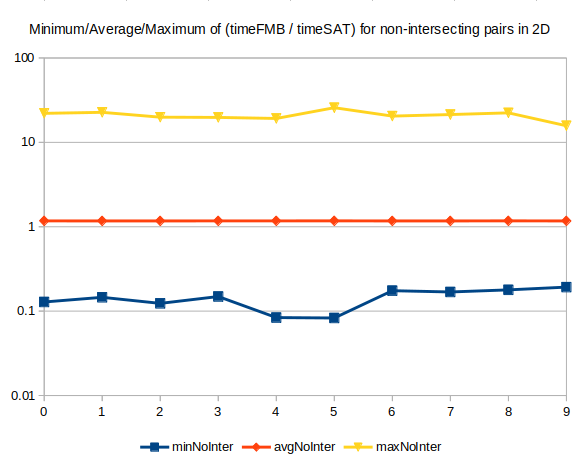
\includegraphics[width=10cm]{./2dnointer.png}\\
\end{figure}
\end{center}

\begin{center}
\begin{figure}[H]
\centering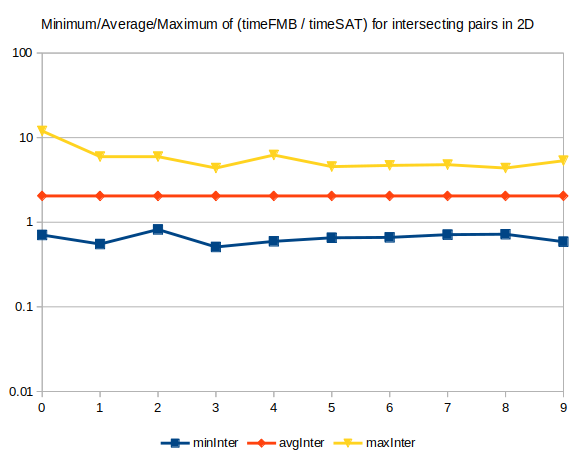
\includegraphics[width=10cm]{./2dinter.png}\\
\end{figure}
\end{center}

\begin{center}
\begin{figure}[H]
\centering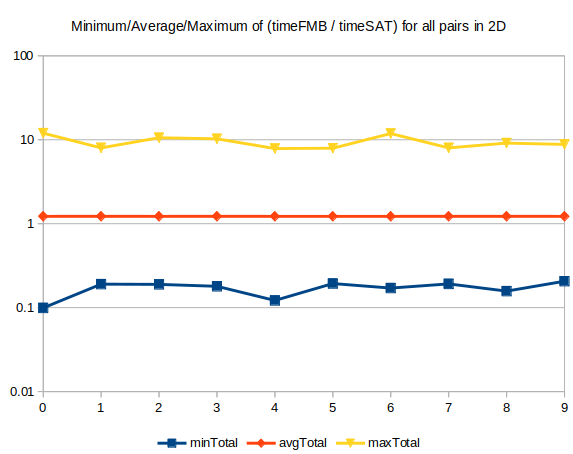
\includegraphics[width=10cm]{./2dtotal.png}\\
\end{figure}
\end{center}

\subsubsection{3D}

\begin{center}
\begin{figure}[H]
\centering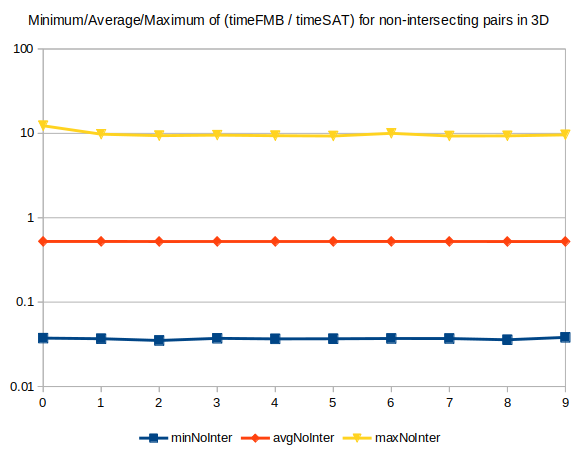
\includegraphics[width=10cm]{./3dnointer.png}\\
\end{figure}
\end{center}

\begin{center}
\begin{figure}[H]
\centering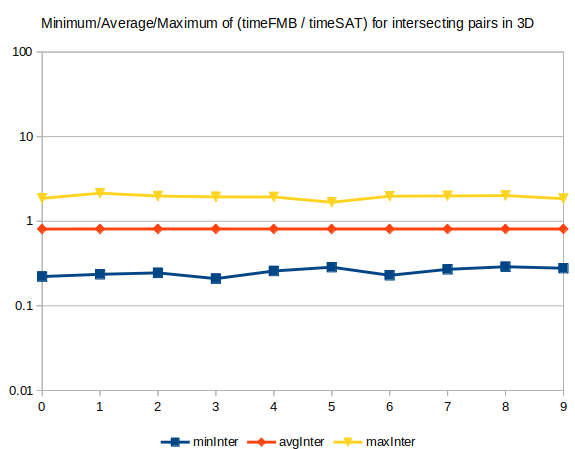
\includegraphics[width=10cm]{./3dinter.png}\\
\end{figure}
\end{center}

\begin{center}
\begin{figure}[H]
\centering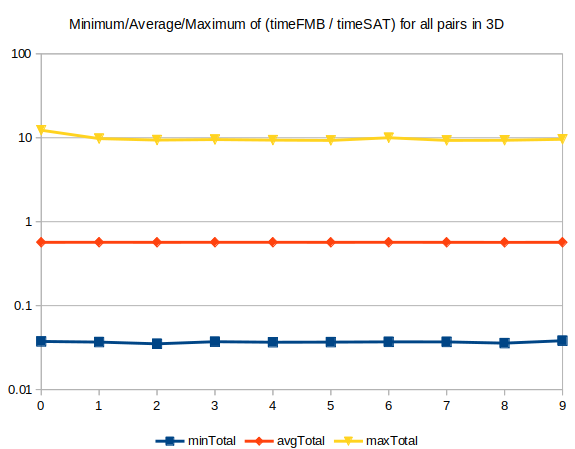
\includegraphics[width=10cm]{./3dtotal.png}\\
\end{figure}
\end{center}

\section{Conclusion}

The validation proves that the FMB algorithm correctly identifies intersection of pairs of Frames in accordance with the results of the SAT algorithm.\\

The qualification proves that the FMB algorithm is in average 50\% slower than the SAT algorithm in 2D, and 17\% faster in 3D.\\

\section{Annex}

\subsection{SAT implementation}
\label{sat_implementation}

In this section I introduce the code of the implementation of the SAT algorithm, used to validate and qualify the FMB algorithm.\\

\subsubsection{Header}

\begin{scriptsize}
\begin{ttfamily}
\verbatiminput{../sat.h}
\end{ttfamily}
\end{scriptsize}

\subsubsection{Body}

\begin{scriptsize}
\begin{ttfamily}
\verbatiminput{../sat.c}
\end{ttfamily}
\end{scriptsize}

\subsection{Makefile}

In this section I introduce the Makefile used to compile the code given in the previous sections.\\

\begin{scriptsize}
\begin{ttfamily}
\verbatiminput{../Makefile}
\end{ttfamily}
\end{scriptsize}

\begin{thebibliography}{9}
\bibitem{fourier} J.J.-B. Fourier. Oeuvres II. Paris, 1890
\bibitem{motzkin} T.S. Motzkin. {\em Beitr\"{a}ge zur Theorie der linearen Ungleichungen}. Thesis, 1936. Reprinted in: {\em Theodore S. Motzkin: selected papers} (D.Cantor et al., eds,), Birkh\"{a}user, Boston, 1983.
\bibitem{SAT} Dynamic Collision Detection using Oriented Bounding
Boxes, David Eberly, Geometric Tools, Redmond WA 98052
\end{thebibliography}

\end{document}
